stm32f4xx-hal contiene una abstracción de hardware multidispositivo además de la API de acceso periférico para los microcontroladores de la serie STMicro STM32F4. La selección de la MCU se realiza mediante puertas de características, generalmente especificadas por cajas de soporte de placa. Las configuraciones admitidas actualmente son:
\begin{tabbing}
	\hspace{120pt}\=\hspace{120pt}\=\hspace{120pt}\=\kill
		\> \textbf{Microcontrolador} \>  \>  \\
	stm32f410 \> stm32f401 \>  stm32f405\> stm32f407\\ 
	stm32f411 \> stm32f412 \> stm32f413 \> stm32f415\\ 
	stm32f417 \> stm32f423 \> stm32f427 \> stm32f429\\ 
	stm32f437 \> stm32f439 \> stm32f446 \> stm32f469\\ 
	stm32f479 \>  \>  \> 
\end{tabbing} 


La idea detrás de esta caja es pasar por alto las ligeras diferencias en los diversos periféricos disponibles en esos MCU para que se pueda escribir un HAL para todos los chips de esa misma familia sin tener que cortar y pegar cajas para cada modelo.

¡La colaboración en esta caja es muy bienvenida, al igual que las solicitudes de extracción!

Esta caja se basa en la fantástica \textbf{crate stm32f4} de \textbf{Adam Greig} para proporcionar definiciones de registro apropiadas e implementa un conjunto parcial de rasgos incrustados.

Parte de la implementación se adaptó descaradamente de la \textbf{crate stm32f1xx-hal} iniciada originalmente por \textbf{Jorge Aparicio}.


\section{Configurando el proyecto}

Compruebe si existe el \textbf{BSP} para su placa en la tabla del microcontrolador. Si existe, la \textbf{crate stm32f4xx-hal} ya debería estar incluida, por lo que puede usar el \textbf{bsp} como \textbf{BSP} para su proyecto.

De lo contrario, cree un nuevo proyecto de Rust como lo hace normalmente con \textbf{cargo init}. El "hola mundo" del desarrollo integrado generalmente consiste en hacer parpadear un LED. El código para hacerlo está disponible en ejemplos \textbf{/delay-syst-blinky.rs}. Copie ese archivo en \textbf{main.rs} de su proyecto.

También necesita agregar algunas dependencias a su \textbf{Cargo.toml}:

\begin{lstlisting}[language=c]
[dependencies]
embedded-hal = "0.2"
nb = "1"
cortex-m = "0.7.3"
cortex-m-rt = "0.7"
# Panic behaviour, see https://crates.io/keywords/panic-impl for alternatives
panic-halt = "0.2"

[dependencies.stm32f4xx-hal]
version = "0.10"
features = ["rt", "stm32f411"] # replace the model of your microcontroller here
\end{lstlisting}

También debemos decirle a Rust cómo vincular nuestro ejecutable y cómo distribuir el resultado en la memoria. Para lograr todo esto, copie \textbf{.cargo/config} y \textbf{memory.x} del repositorio \textbf{stm32f4xx-hal} a su proyecto y asegúrese de que los tamaños coincidan con la hoja de datos. También tenga en cuenta que puede haber diferentes tipos de memoria que no son iguales; para estar seguro, solo especifique el tamaño del primer bloque en la dirección especificada.


\section{Encendiendo un LED en la tarjeta STM32F411RE}

Para controlar el GPIO de la tarjeta stm32F411RE primero debemos configurar el archivo \textbf{Cargo.toml} 

\begin{lstlisting}[language=c]
#Archivo Cargo.toml
[package]
name = "prender_led2"
version = "0.1.0"
edition = "2021"

[dependencies]
embedded-hal = "0.2"
nb = "1"
cortex-m = "^0.7"
cortex-m-rt = "^0.6"
rtt-target = { version =  "0.3.1", features = ["cortex-m"] }
panic-halt = "0.2"

[dependencies.stm32f4xx-hal]
version = "0.10"
features = ["rt", "stm32f411"] 
\end{lstlisting}

Ahora es necesario crear el \textbf{Embed.toml} en el mismo directorio donde se encuentra el directorio \textbf{Cargo.toml}.

\begin{lstlisting}[language=c]
# Archivo Embed.toml
[default.probe]
protocol = "Swd"

[default.general]
chip = "STM32F411RETx" # uncomment this line for micro:bit V2
# chip = "nrf51822_xxAA" # uncomment this line for micro:bit V1

[default.rtt]
enabled = true

[default.gdb]
enabled = false	
\end{lstlisting}

En el mismo directorio también se crea un archivo llamado \textbf{memory.x} en donde se escribe la distribución de memoria del microcontrolador stm32f411re

\begin{lstlisting}[language=c]
MEMORY
{
	/* NOTE K = KiBi = 1024 bytes */
	FLASH : ORIGIN = 0x08000000, LENGTH = 512K
	RAM : ORIGIN = 0x20000000, LENGTH = 128K
}
/* This is where the call stack will be allocated. */
/* The stack is of the full descending type. */
/* NOTE Do NOT modify `_stack_start` unless you know what you are doing */
_stack_start = ORIGIN(RAM) + LENGTH(RAM);
\end{lstlisting}

El siguiente archivo para crear \textbf{build.rs} para procesar el archivo de memoria \textbf{memory.x}.

\begin{lstlisting}[language=c]
// Archivo build.rs
use std::env;
use std::fs::File;
use std::io::Write;
use std::path::PathBuf;

fn main() {
	// Put `memory.x` in our output directory and ensure it's
	// on the linker search path.
	let out = &PathBuf::from(env::var_os("OUT_DIR").unwrap());
	File::create(out.join("memory.x"))
	.unwrap()
	.write_all(include_bytes!("memory.x"))
	.unwrap();
	println!("cargo:rustc-link-search={}", out.display());
	
	// By default, Cargo will re-run a build script whenever
	// any file in the project changes. By specifying `memory.x`
	// here, we ensure the build script is only re-run when
	// `memory.x` is changed.
	println!("cargo:rerun-if-changed=memory.x");
}
\end{lstlisting} 

Ahora se crea un directorio llamado \textbf{.cargo} en donde creamos un archivo llamado \textbf{config}, dicho archivo nos permite compilar y enlazar nuestro proyecto


\begin{lstlisting}[language=c]
[target.thumbv7em-none-eabihf]
runner = 'probe-run --chip STM32F411CEUx'
rustflags = [
"-C", "link-arg=-Tlink.x",
]

[build]
target = "thumbv7em-none-eabihf"	
\end{lstlisting}


Ahora se modifica el archivo \textbf{src/main.rs} 

\begin{lstlisting}[language=c]
// ************ Archivo src/main.rs ****************
#![deny(unsafe_code)]
#![allow(clippy::empty_loop)]
#![no_main]
#![no_std]

// Halt on panic
use panic_halt as _; // Manejador de panic 

use cortex_m_rt::entry;
use stm32f4xx_hal as hal;

use crate::hal::{pac, prelude::*};
use rtt_target::{rtt_init_print, rprintln};


#[entry]
fn main() -> ! {
	rtt_init_print!();
	rprintln!("Prendiendo Led Cada Segundo");
	if let (Some(dp), Some(cp)) = (
	pac::Peripherals::take(),
	cortex_m::peripheral::Peripherals::take(),
	) {
		// Configuracion del led de la tarjeta stm32f411 
		let gpioa = dp.GPIOA.split();
		let mut led = gpioa.pa5.into_push_pull_output();
		
		// configuracion del reloj de la tarjeta a 48Mhz
		let rcc = dp.RCC.constrain();
		let clocks = rcc.cfgr.sysclk(48.mhz()).freeze();
		
		// Creacion del retardo con SysTick
		let mut delay = hal::delay::Delay::new(cp.SYST, &clocks);
		loop {
			// On for 1s, off for 1s.
			led.set_high();
			delay.delay_ms(2000_u32);
			led.set_low();
			delay.delay_ms(1000_u32);
		}       
		
	}
	loop{}
}
\end{lstlisting}

La estructura del proyecto se muestra en la figura \ref{cap3:001}

\begin{figure}[htb]
	\centering
	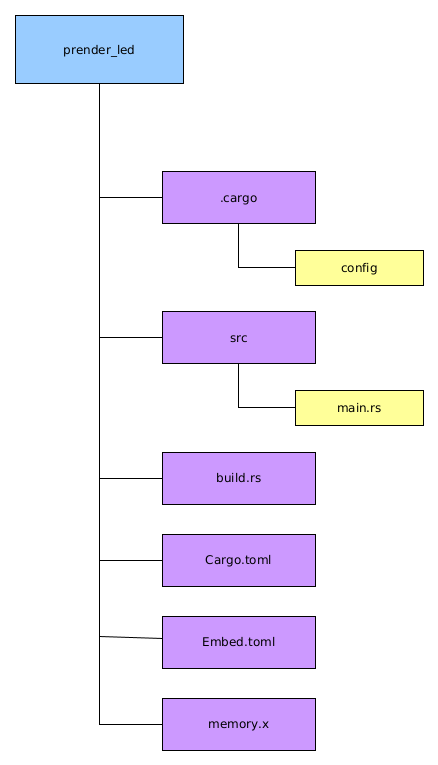
\includegraphics[width=0.3\textwidth]{capitulo3/prender_led.png}
	\caption{Estructura general del proyecto para controlar GPIO}
	\label{cap3:001}
\end{figure} 

Ahora si ejecutamos el comando:

\begin{lstlisting}[language=c]
cargo embed --target thumbv7em-none-eabihf	
\end{lstlisting}

La salida obtenida por dicho comando se muestra en la figura 

\begin{figure}[htb]
	\centering
	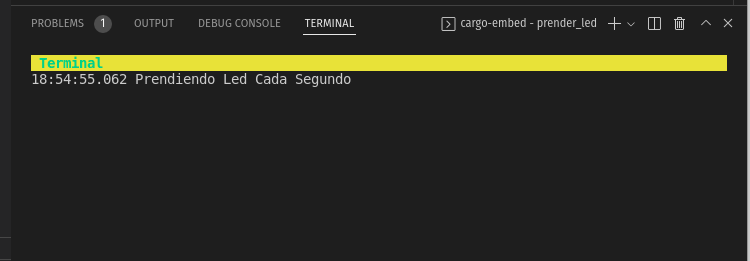
\includegraphics[width=0.6\textwidth]{capitulo3/salida_prender_led.png}
	\caption{Salida en la terminal el ejecutar el proyecto}
	\label{cap3:002}
\end{figure} 


\section{Controlando un bus de GPIO}

Para controlar los GPIO del microcontrolador necesitamos conocer los nombres de estos pines


\begin{figure}[htb]
	\centering
	\subfloat[Izquierdo]{
		\label{cap3:003_I}
		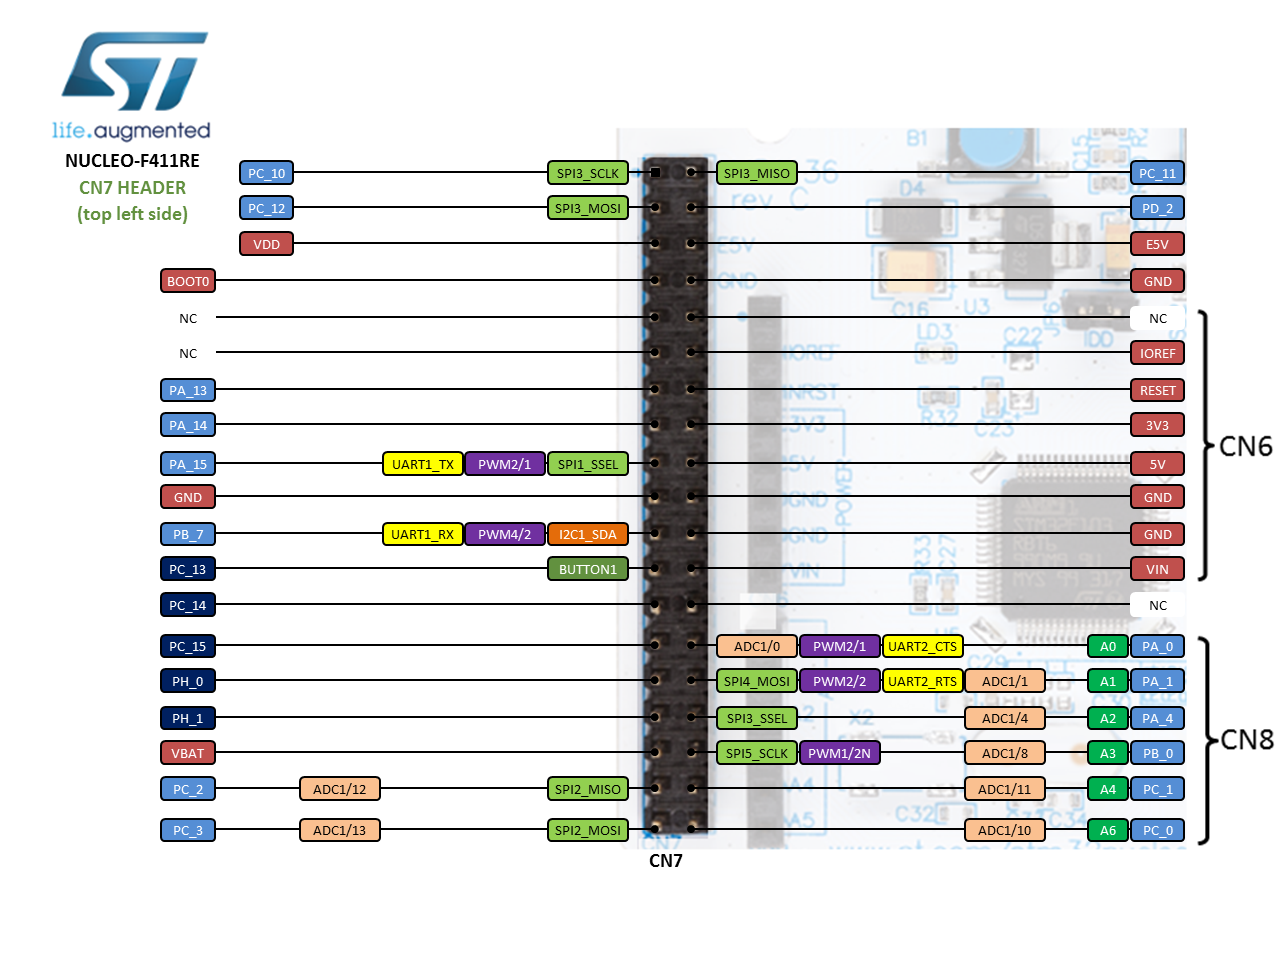
\includegraphics[width=0.5\textwidth]{capitulo3/nucleo_f411re_1.png}}
	\subfloat[Derecho]{
		\label{cap3:003_D}
		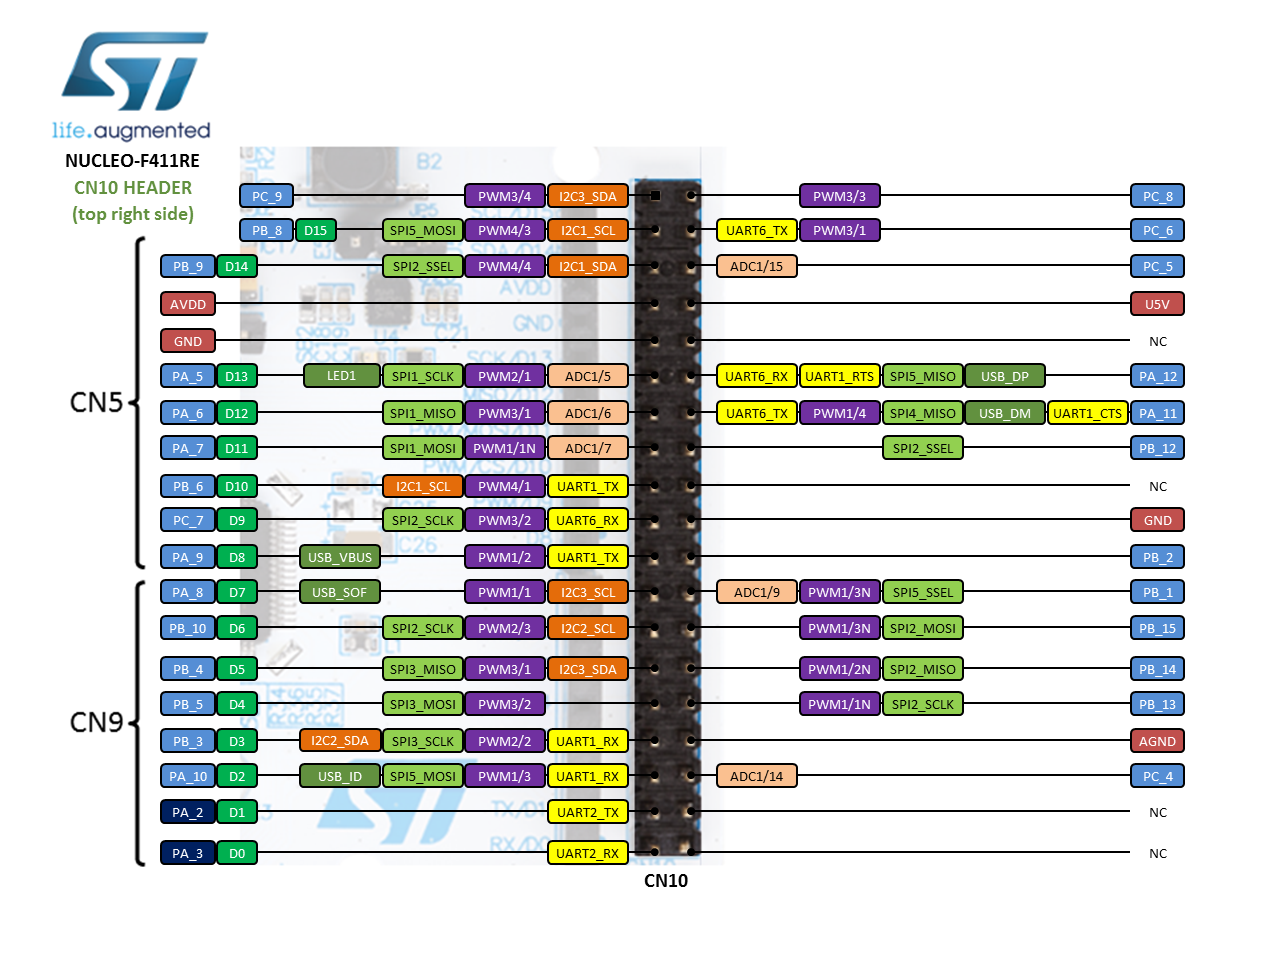
\includegraphics[width=0.5\textwidth]{capitulo3/nucleo_f411re_2.png}}
	\caption{Pins de la tarjeta núcleo F411RE}
	\label{cap3:003}
\end{figure}

De la figura \ref{cap3:003} vamos a tomar los pines del lado derecho para la creación del bus. Los pines van a ser (PA\_5, PA\_6, PA\_7, PA\_9) y llamaremos a este bus BCD \footnote[1]{Los pines se pueden observar claramente en la figura \ref{cap3:003_D}}.

